\section{Systemmodelle}

\subsection{Anwendungsfalldiagramme}

\subsubsection*{Kartenansicht}
\noindent\makebox[\textwidth]{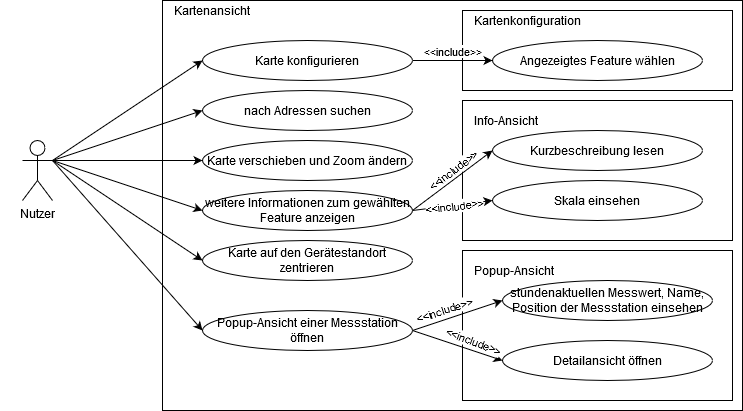
\includegraphics[width=\textwidth]{Anwendungsfalldiagramm_Kartenansicht.png}}

\subsubsection*{Detailansicht}
\noindent\makebox[\textwidth]{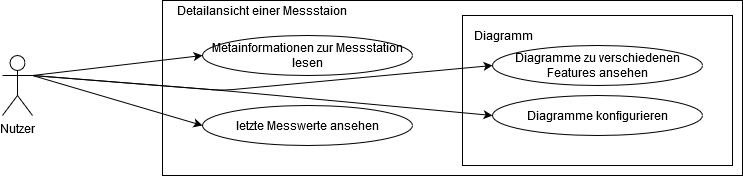
\includegraphics[width=\textwidth]{Anwendungsfalldiagramm_Detailansicht.png}}
\newpage

\subsection{Ablaufdiagramm}

\noindent\makebox[\textwidth]{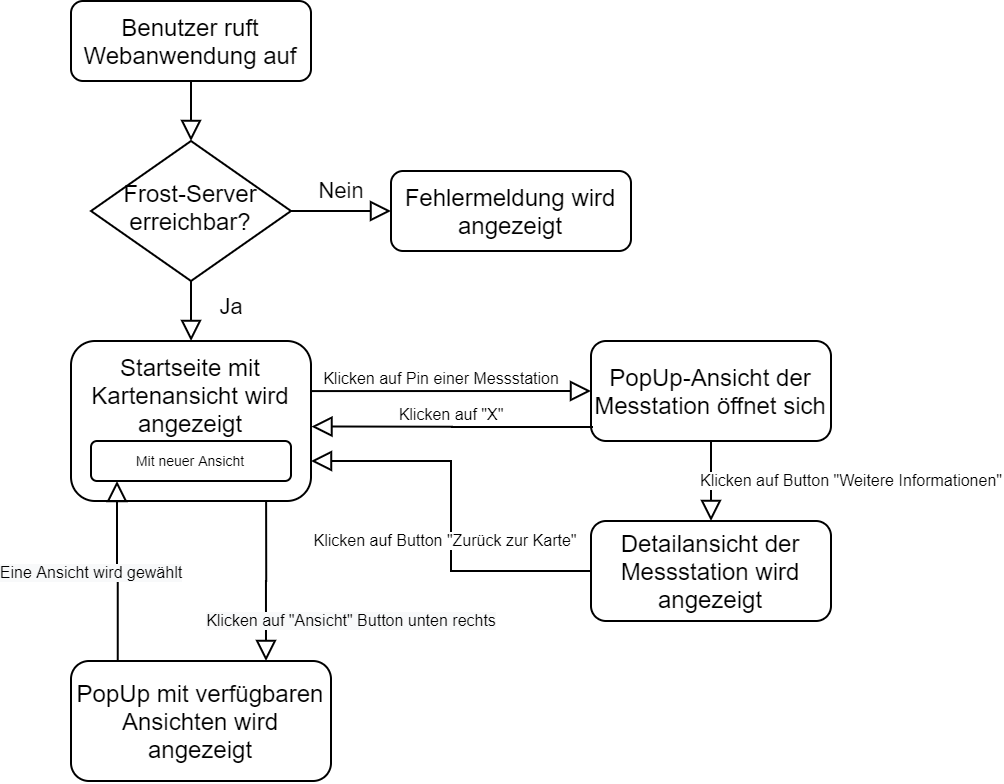
\includegraphics[width=\textwidth]{Ablaufdiagramm.png}}

\subsection{Szenarios}

\subsubsection*{Szenario 1: Ansicht, der studenaktuellen Feinstaubwerte (PM 10) am Smartphone}
\textbf{Nutzer:} Nutzer mit grundlegenden IT-Kenntnissen der schon einmal ähnliche Anwendungen bedient hat (z.B. Google Maps) 
und somit intuitiv die Karte bedienen kann. Des Weiteren hat er jedoch wenig Kenntnisse über Feinstaubwerte und benötigt somit 
eine Einordnung und Erklärung der \glspl{Messwert}.

\textbf{Beschreibung:} Der Nutzer interessiert sich für die aktuellen Feinstaubwerte in seiner Stadt.

\textbf{Konkreter Ablauf:}
Der Nutzer öffnet die \gls{Webanwendung}, indem er die URL der \gls{Webanwendung} in seinen Smartphone Browser eingibt und bestätigt. Daraufhin öffnet 
sich die Kartenansicht der Anwendung. Dort sind die \glspl{Station} als Punkt eingetragen. Über einen Button in der rechten unteren 
Ecke ruft der Nutzer das Konfigurationsmenü der Karte auf. Dort Klickt er auf PM 10 (Feinstaub). Daraufhin werden nur die 
\glspl{Station} als Punkt auf der Karte angezeigt, die das \gls{Feature} PM10 messen und sie werden, aufgrund ihres zuletzt 
gemessenen PM10 Wertes eingefärbt. Desto grüner ein Punkt, desto niedriger der Wert. Desto roter ein Punkt, desto höher ein Wert. 
Die Farbskala wird in der linke unteren Ecke angezeigt.
Um einen \gls{Messwert} in Zahlenform einer \gls{Station} anzuzeigen, klickt der Nutzer auf einen Punkt. Daraufhin öffnet am 
unteren Bildschirmrand eine Popup-Ansicht, in der der Name der \gls{Station}, die Position und der PM10 Wert angezeigt wird. 
Außerdem wird eine Warnung angezeigt, wenn der \gls{Messwert} einen Grenzwert überschritten hat.
\newpage

\subsubsection*{Szenario 2: Ansicht der Diagramme einer spezifischen Messstation am Computer}
\textbf{Nutzer:} Nutzer mit grundlegenden IT-Kenntnissen der schon einmal ähnliche Anwendungen bedient hat (z.B. Google Maps) 
und somit intuitiv die Karte bedienen kann. Er hat sich schon häufiger über Luftqualität informiert und ist an konkreten 
\glspl{Messwert}n und deren zeitlicher Entwicklung interessiert.

\textbf{Beschreibung:} Der Nutzer möchte Diagramme einer \gls{Station} einsehen.

\textbf{Konkreter Ablauf:} Der Nutzer öffnet die \gls{Webanwendung}, indem er die URL der \gls{Webanwendung} in in den Browser seines Computer eintippt 
und bestätigt. Daraufhin öffnet sich die Kartenansicht der \gls{Webanwendung}. Über das Suchfeld in der linken oberen Ecke gibt 
er eine Adresse ein oder klickt auf den Button zur Standortbestimmung. Daraufhin zentriert sich die Karte auf den genwünschten Ort. 
Der Nutzer klickt nun auf einen Punkt in der Nähe, der die gesuchte \gls{Station} repräsentiert. Nun öffnet sich ein Popup neben 
dem Punkt. Darin wird der Name der \gls{Station}, ihre Position und ihr letzter \gls{Messwert} des ausgewählten \gls{Feature} 
angezeigt, der in der Kartenkonfiguration eingestellt ist. Des Weiteren, wird ein Button angezeigt, auf dem "weitere Informationen" 
steht. Der Nutzer klickt auf den Button.
Daraufhin wird die Profilansicht der \gls{Station} angezeigt. In der linken oberen Ecke wird der Name und Metainformationen 
der \gls{Station} angezeigt. In der rechten oberen Ecke wird eine statische Karte angezeigt, auf der die Position der \gls{Station} 
markiert ist.
Darunter werden Diagramme zu den gemessenen Features der \gls{Station} angezeigt. Die angezeigten Diagramme sind von \gls{Station} 
zu \gls{Station} unterschiedlich, da die \glspl{Station} unterschiedliche Features messen.